\section{Results}

\subsection{Data usage across operating systems and scenarios}

Total network data usage across all operating systems and applicable scenarios for performed tasks, is presented on charts in Figures~\ref{fig-setup-chart}--\ref{fig-apps-chart}. To keep the results comparable and avoid dominance by bulk transfers, we excluded traffic to domains used for app and system update payload delivery (large binary downloads), though this exclusion was not perfect and some residual update-related traffic remains in the dataset. Generally, we expect lower network traffic in configurations with fewer Google services present.

\begin{figure}
	\includegraphics[width=\textwidth]{images/setup-data-usage.eps}
	\caption{Task 0: Initial setup data usage} \label{fig-setup-chart}
\end{figure}

Figure \ref{fig-setup-chart} illustrates network activity during initial device setup. As expected, stock Android shows the highest data usage. The modest reductions between privacy-adjusted scenarios indicate that configuration choices provide little control over automatic updates and background synchronization. Across all distributions, variations align with service architecture: configurations incorporating more Google services generate proportionally higher traffic, while de-Googled baselines demonstrate substantially reduced exchange. LineageOS with official Google Play Services generates substantially less traffic than stock Android due to its more minimal base system, yet remains considerably higher than configurations without proprietary Google services, with the microG variant and Google-free installation achieving notable further reductions. On GrapheneOS, Scenario B demonstrates that even when sandboxed Google Play Services are installed and granted network and background permissions, they remain largely inactive when not deliberately invoked, contrasting with the persistent background activity characteristic of integrated GMS deployments.

\begin{figure}
	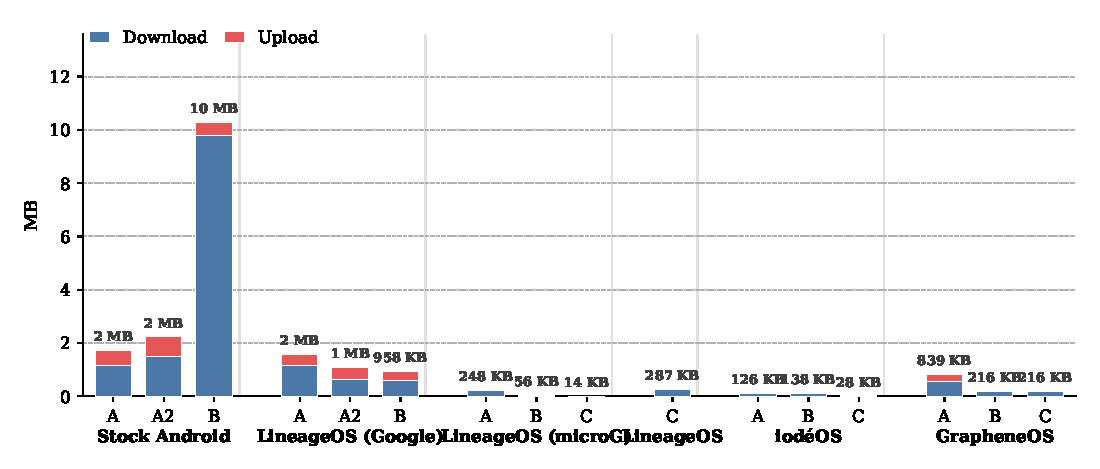
\includegraphics[width=\textwidth]{images/idle-data-usage.eps}
	\caption{Task 1: Idle data usage} \label{fig-idle-chart}
\end{figure}

Network activity observed during system idle following a reboot is presented in Figure \ref{fig-idle-chart}. Stock Android again shows the highest data usage, though Scenario B exhibits unexpectedly elevated traffic compared to both Scenario A2 and Scenario A. This anomaly stems from substantial background communication with www.gstatic.com, likely triggered by automatic updates or application background activity during the measurement time.

LineageOS in Scenario C similarly deviate from anticipated patterns, generating more idle traffic than its microG variant. LineageOS made connections to agnss.goog (Google Assisted GNSS) and www.gstatic.com. The agnss.goog endpoint was also observed in LineageOS (microG) during other measurement tasks, indicating that the entire LineageOS family retains this Google-dependent location mechanism. Other alternative distributions either replace this component with independent implementations or allow users to disable it entirely. GrapheneOS exhibits virtually identical idle traffic in Scenarios B and C, confirming that sandboxed Google Play Services remain dormant when not actively invoked.

\begin{figure}
	\includegraphics[width=\textwidth]{images/apps-data-usage.eps}
	\caption{Task 2: Basic apps interactions data usage} \label{fig-apps-chart}
\end{figure}

Figure~\ref{fig-apps-chart} shows network activity during basic app interactions that should not require Internet connectivity. Stock Android dominates with substantial data usage mostly by uncontrolled updates. All alternative distributions demonstrate dramatically lower traffic, with de-Googled configurations remaining effectively silent. Notably, whenever official Google Play Services were present and a Google account logged in at least a single request to Google infrastructure occurred.

\subsection{Domain distribution and Google dependencies}

\begin{figure}
	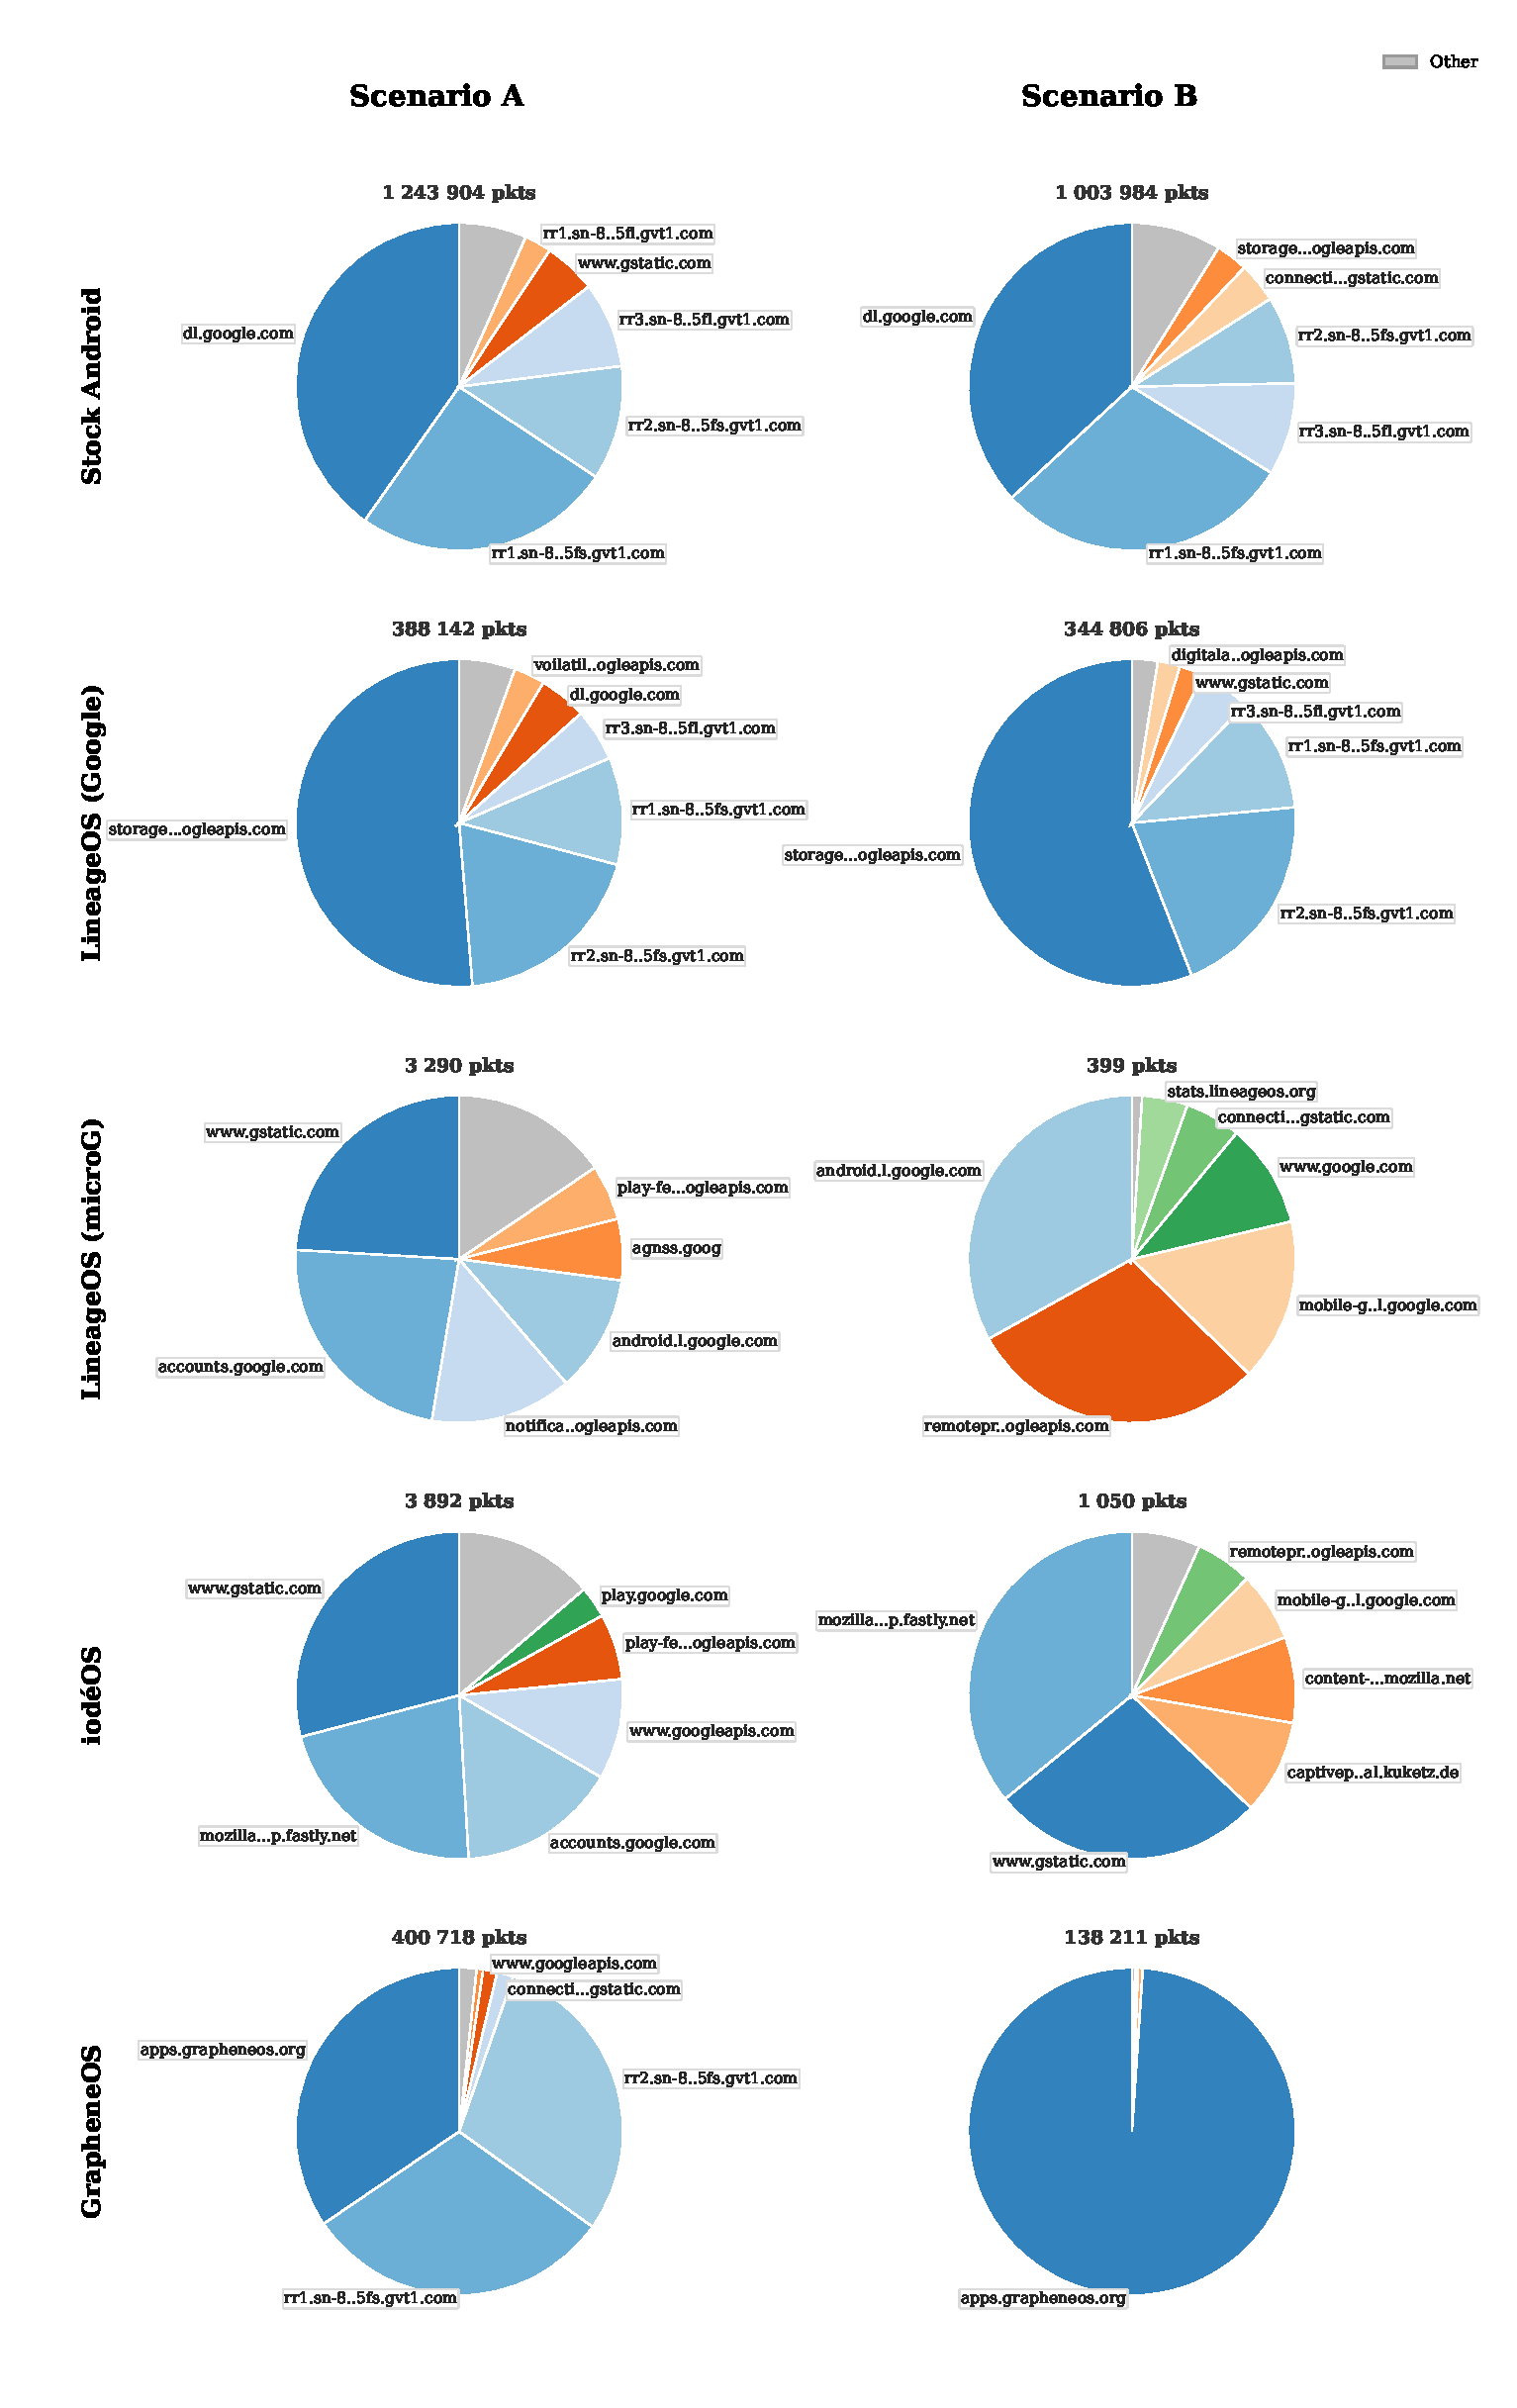
\includegraphics[width=\textwidth]{images/domains.eps}
	\caption{Domain-level distribution of network packets for scenarios A (with Google account) and B (without Google account, but Google Services present), aggregated over all tasks. Each pie shows the top domains by packet count for a given operating system and scenario.} \label{fig-domains-chart}
\end{figure}

Figure \ref{fig-domains-chart} presents the domain-level distribution of network traffic for Scenarios A and B. They were selected as the most realistic configurations incorporating essential Google functionality while differing in account linkage and privacy-related settings. Overall traffic is dominated by large content transfers, as systems download necessary resources and updates. Stock Android contacts the widest range of Google domains, spreading traffic across many different endpoints. Alternative systems show less Google communication, though patterns vary by design. GrapheneOS makes more requests than microG-based systems because it downloads Google services on demand from its own app store rather than having them preinstalled. IodéOS and LineageOS with microG reach fewer Google servers overall, as microG minimizes Google connectivity while still enabling basic features. IodéOS additionally relies on some Mozilla infrastructure not present in other systems.

Table~\ref{tab:domains-mechanisms} shows the infrastructure dependencies for basic system functions. LineageOS variants remain closest to stock Android, relying entirely on Google servers for connectivity checks, remote provisioning, and location assistance. IodéOS adopts an intermediate position, using independent infrastructure for connectivity checks while still depending on Google for remote provisioning and location services. GrapheneOS demonstrates the strongest de-Googling, substituting all three functions with its own or independently operated infrastructure. Both iodéOS and GrapheneOS expose these mechanisms through explicit system settings toggles, though GrapheneOS offers more granular control: users may choose between its independent proxy infrastructure and official Google servers for each function, with defaults configured to avoid Google connections entirely.

\begin{table}
	\caption{Domains observed for connectivity check, remote provisioning, and location assistance.}\label{tab:domains-mechanisms}
	\centering
	\resizebox{\linewidth}{!}{%
		\begin{tabular}{|l|l|l|l|}
			\hline
			System & Connectivity check & Remote provisioning & Location assistance\\
			\hline
			Stock Android & connectivitycheck.gstatic.com & -- & supl.google.com agnss.goog\\
			LineageOS & connectivitycheck.gstatic.com & remoteprovisioning.googleapis.com & supl.google.com agnss.goog\\
			iodeOS & captiveportal.kuketz.de & remoteprovisioning.googleapis.com & supl.google.com\\
			GrapheneOS & connectivitycheck.grapheneos.network & remoteprovisioning.grapheneos.org & gs-loc.apple.grapheneos.org\\
			\hline
		\end{tabular}%
	}
\end{table}


\subsection{Additional findings}

[Mention that some of these results where gathered earlier on android 14, we where not able to confirm them later in android 16 due to frida method not working anymore, but we expect general trend to remain similar]

NOTES FOR: Android “checkin” request:
in stock os sends real imei and serial number.
in microg fake and randomly changing imei and mac adress is used.
mac addresses start with "b4:07:f9" but last part varies, all imei starts with 35503104...
android id in microg requests is often empty, zero.
microg sends real device information like device model, os version, timezone.
microg sends serial key like 008741D1E2C1C2C7, which is also displayed in microg settings, it acts as a unique generated identifier to hide real device identifiers.

NOTES FOR: app-measurment.com/region1.app-measurement.com
on os with google services we noticed requests to these domains. on lineage stock and graphene. these requests contain app name, source of installation (google play/aurora/manual), system theme (dark/light), app version, android id. Info about installed and not open apps where send too. We where not able to verify what region1.app-measurement.com on graphene os contained because grapheneos blocked frida attempts.

NOTES FOR: ADID
In few requests in stock we noticed ADID (format: d72ed0d9-c534-4c76-bf42-5185a6e7850d). It was present in some google requests to different domains. value was constant across requests. It is resettable in settings, after removing it in settings we noticed it being changed into zeros.

NOTES FOR: Microg location
microG is sending nearby cell-tower and Wi‑Fi scan data to api.positon.xyz to estimate the phone’s location (network-based geolocation). The cell-tower request succeeds and returns an approximate lat/lng with accuracy, while the Wi‑Fi-based lookups return “404 Not found,” meaning that service/key doesn’t have matching Wi‑Fi AP location data available.
It happens only after users enables it and chooses location provider. No google.
<request base64="false"><![CDATA[POST /v1/geolocate?key=627db168-2a5e-11ef-afbd-a75f87425aa4 HTTP/1.1
User-Agent: microG/0.3.10.250932 (Linux; Android 16; com.google.android.gms)
Content-Type: application/json; charset=utf-8
Host: api.positon.xyz
Connection: keep-alive
Accept-Encoding: gzip, deflate, br
Content-Length: 298

{"considerIp":false,"homeMobileCountryCode":260,"homeMobileNetworkCode":1,"radioType":"wcdma","cellTowers":[{"radioType":"wcdma","mobileCountryCode":260,"mobileNetworkCode":1,"locationAreaCode":11018,"cellId":75678399,"age":16,"psc":355,"signalStrength":-94}],"fallbacks":{"lacf":true,"ipf":false}}]]></request>
<status>200</status>
<responselength>532</responselength>
<mimetype>JSON</mimetype>
<response base64="false"><![CDATA[HTTP/2 200 OK
Server: nginx/1.22.1
Date: Thu, 11 Dec 2025 10:49:24 GMT
Content-Type: application/json; charset=utf-8
Content-Length: 322
X-Powered-By: Express
Etag: W/"142-LUquWahK9inoXp0ExE4zfupVysQ"

{"raw":[{"timestamp":1772928000000,"location":{"lat":53.044937,"lng":21.585724},"accuracy":3294,"cellTower":{"radioType":"wcdma","mobileCountryCode":260,"mobileNetworkCode":1,"locationAreaCode":11018,"cellId":75678399,"age":16,"psc":355,"signalStrength":-94}}],"location":{"lat":53.044937,"lng":21.585724},"accuracy":3294}]]></response>


\subsection{Google Takeout}